%%
%% 2019 07 04 Ph. G. Freimann
%%

\section{Funktionen}\index{Funktion|textbf}
\sectuntertitel{longitudo, latitudo (Begriffe nach Nikolaus von Oresme)}
%%%%%%%%%%%%%%%%%%%%%%%%%%%%%%%%%%%%%%%%%%%%%%%%%%%%%%%%%%%%%%%%%%%%%%%%%%%%%%%%%
\subsection*{Lernziele}

\begin{itemize}
 \item Zuordnung
 \item Mengenbegriffe: Definitionsmenge (= Definitionsbereich) vs. Quellbereich
 \item Wertebereich (= Bildmenge) vs. Wertevorrat (= Zielmenge)
 \item Darstellungsarten
   \begin{itemize}
      \item Wertetabelle
      \item Graphen
      \item Funktionsterm
   \end{itemize}
 \item verschiedene Notationen
 \item Gleichungen visualisieren
 \item Achsen
 \item Funktionsgleichung
 \item Abhängige, unabhängige Variable / Argument, Parameter, Funktionswert
\end{itemize}

%%\TALS{(\cite{frommenwiler17alg} S.161 (Kap. 3))}
%%\GESO{(\cite{marthaler21alg}       S.211 (Kap. 13))}

\TadBMTA{211}{13}
\newpage
\subsection{Allgemeiner Funktionsbegriff\GESO{ (optional)}}\index{Funktion!allgemeiner Begriff}
Mengenbezeichnungen bei Gleichungen (Diese Mengen sind bereits
bekannt\footnote{Die Definitionsmenge bezeichnet hier die Menge aller
  Zahlen für die alle Terme definiert sind.}):

\begin{tabular}{cp{4cm}l}
  \raisebox{-3cm}{\includegraphics[width=8cm]{allg/funktionen/img/MengenbezeichnungenBeiGleichungen.png}}
  & Beispiel & \TRAINER{\makecell{$\frac{1}{x-3}=5$\\
  $\Grundmenge=\mathbb{R}$\\
  $\DefinitionsMenge{}=\mathbb{R}\backslash{}\{3\}$\\
      $\lx = \{3.2\}$}%% end makecell
    }%% END Trainer
\end{tabular}

\vspace{6mm}

Mengenbezeichnungen bei Funktionen:
\TRAINER{\begin{center}
  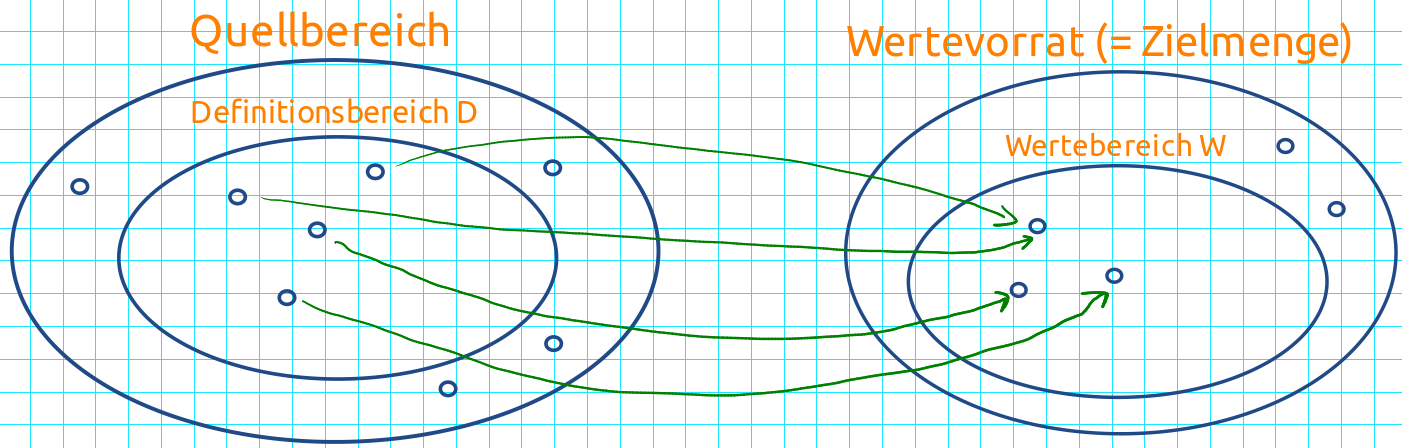
\includegraphics[width=16cm]{allg/funktionen/img/MengenbezeichnungenBeiFunktionen.png}
\end{center}
}%% END TRAINER

\noTRAINER{\begin{center}
  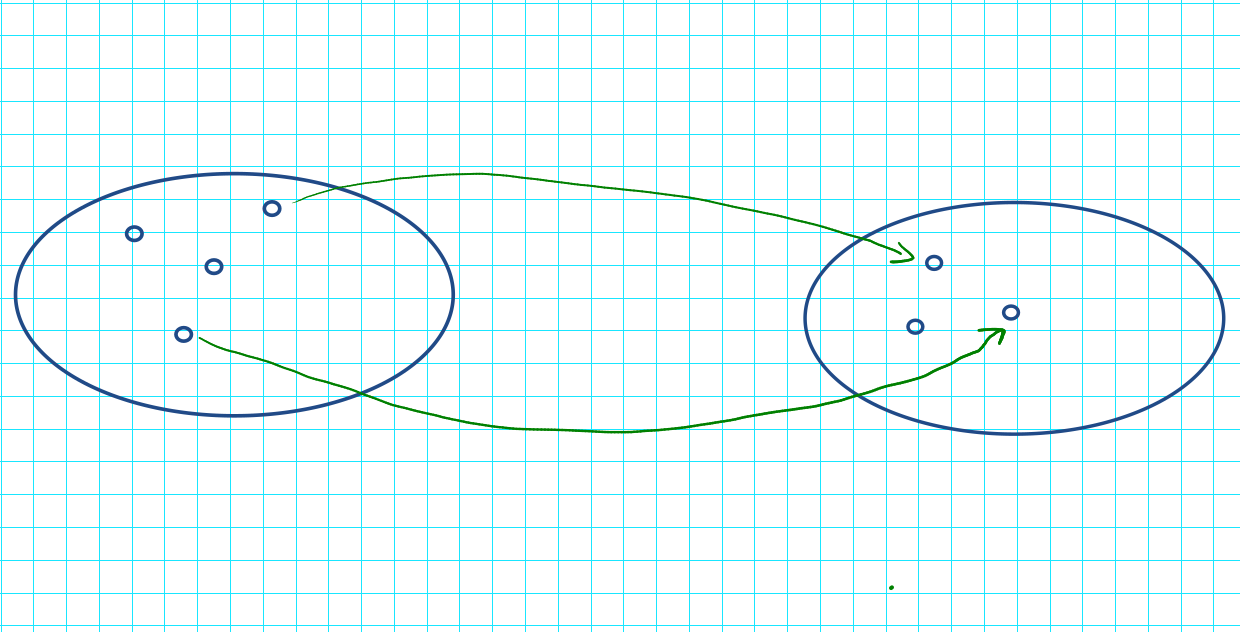
\includegraphics[width=16cm]{allg/funktionen/img/MengenbezeichnungenBeiFunktionenLeer.png}
\end{center}
}%% END no TRAINER

\newpage
\subsubsection{Definition Funktionsbegriff\GESO{ (optional)}}

\begin{definition}{Funktion}{}\index{Funktion!Definition}
    Eine \textbf{Funktion}\index{Funktion} ist eine eindeutige \textbf{Zuordnung}\index{Zuordnung}, die jeder Zahl
    $x$ aus einem Definitionsbereich \textbf{genau} eine Zahl $y$ aus
    einem Wertevorrat\index{Wertevorrat} (=
    Zielmenge)\index{Zielmenge} zuordnet.

    $$f: \mathbb{D} \mapsto{} \mathbb{W}$$
\end{definition}

\TRAINER{Hier Graphen von Funktionen zeigen (\zB OLAT).}

\TALS{
\begin{beispiel}{reelle Funktion}{}
  Funktion Sinus $\sin()$:
  $\DefinitionsMenge{} = \mathbb{R}$; $\Wertebereich{}= [-1; 1]$
  $$\sin: \mathbb{R} \rightarrow [-1; 1] \text{ mit } \varphi\mapsto{}\sin(\varphi) $$
\end{beispiel}

\begin{beispiel}{}{}
  Funktion Tangens $\tan()$:
  $\DefinitionsMenge{} = \mathbb{R}\backslash\{\pm{}90^\circ, \pm{}270^\circ, \pm{}450^\circ, ...\}$; $\Wertebereich{}= \mathbb{R}$
    
  $$\tan: \mathbb{R}\backslash\{90^\circ{}+z\cdot{}180^\circ{}|z \in \mathbb{Z}\} \rightarrow \mathbb{R} \text{ mit } \alpha\mapsto{}\tan(\alpha) $$
\end{beispiel}
}%% end TALS


\begin{bemerkung}{}{}
  Zum Wertebereich: Wo der Begriff Quellbereich (eine theoretische Obermenge
  des \textbf{Definitionsbereichs}\index{Definitionsbereich}) kaum praktische Bedeutung hat,
  wird jedoch in speziellen Fällen statt dem Wertebereich der
  Wertevorrat\index{Wertevorrat}\footnote{Der Wertevorrat
    wird auch Zielbereich, Zielmenge\index{Zielmenge},
    Cobereich\index{Cobereich} oder Nachbereich\index{Nachbereich}
    genannt (\cite{FormelnUndTafeln19}).}
  angegeben; meist daher, weil der
  Wertebereich in komplexen, fraktalen, sprungstetigen oder sonst wie komplizierten Funktionen schlicht
  und ergreifend nicht bekannt ist.\footnote{\textbf{Beispiel 1}: Bei der Funktion
    «mittlere Tagestemperatur» ist zwar der Wertevorrat ($\mathbb{R}[{}^\circ]$)
    bekannt, jedoch sind die effektiv getroffenen Bildwerte meist nur
    zwischen $-40^\circ$ und $+50^\circ$ vorzufinden (daher ist der
    effektiv eintretende Wertebereich erst dann bekannt, wenn das Wetter
    bereits eingetreten ist bzw. auch gemessen wurde). \\
    \textbf{Beispiel 2}: (Sei $\pi$ die Kreiszahl.) Der Funktion $f: n\mapsto f(n)$; $\mathbb{N} \rightarrow \{0, 1, 2, 3, ..., 9\} \text{mit} f(n) = $
    «millionste Nachkommastelle von $n\pi$»
    kann der effektive Wertebereich nicht
  angesehen werden, bevor wir genügend oft die millionste Ziffer von
  $n\pi$ berechnet haben. Auch hier ist vorerst nur der Wertevorrat, nicht
  aber der Wertebereich bekannt.}
\end{bemerkung}



\GESO{%%
\olatLinkArbeitsblatt{Funktionsbegriff}{https://olat.bms-w.ch/auth/RepositoryEntry/6029794/CourseNode/108030908300504}{Aufgabe
  1.2 (1.1 optional)}
}%% end GESO


\TALS{%%
\olatLinkArbeitsblatt{Funktionsbegriff}{https://olat.bms-w.ch/auth/RepositoryEntry/6029786/CourseNode/108030908410625}{Aufgabe
  1.2 (1.1 optional)}
}%% end GESO

\newpage


\subsection{Arten der Darstellung}
\begin{itemize}
\item Wertetabelle\index{Wertetabelle}:

  \begin{tabular}{c|cccccc}$x$ & -2 & -1 & 0 & 1 & 2 & 2.5\\
    \hline\\
    $f(x)=y=x^2-1$ & \LoesungsRaumKurz{3} & \LoesungsRaumKurz{0} & \LoesungsRaumKurz{-1} & \LoesungsRaumKurz{0} & \LoesungsRaumKurz{3} & \LoesungsRaumKurz{5.25}\\ 
\end{tabular}
\item \textbf{Graphen}\index{Graph} im rechtwinkligen Koordinatensystem
  
\noTRAINER{\bbwGraph{-3}{4}{-1.5}{6}{}}
\TRAINER{  \bbwFunction{-3}{4}{-1.5}{6}{\x*\x - 1 }{-2:2.5}}

\item Funktionsschreibweise (verschiedene Notationen)\\

Funktionsgleichung...:
\noTRAINER{\vspace{15mm}}\TRAINER{$$y=x^2-1$$}

... mit Namen:
\noTRAINER{\vspace{15mm}}\TRAINER{$$f(x)=x^2-1$$}
\noTRAINER{\vspace{15mm}}\TRAINER{$$f:\,\,\, y = x^2-1$$}

Funktionsvorschrift:
\noTRAINER{\vspace{15mm}}\TRAINER{$$x \mapsto x^2-1$$}

\end{itemize}
\newpage

\subsubsection{Definitions- und Wertemenge}

\begin{definition}{Definitionsmenge $\mathbb{D}$}{}
  
Mit \textbf{Definitionsmenge}\index{Definitionsmenge|textbf} $\mathbb{D}$ (auch
Definitionsbereich\index{Definitionsbereich|textbf}) wird die Menge aller
möglichen Funktionsargumente bezeichnet, kurz alle Zahlen, die für $x$
eingesetzt werden dürfen. 
\end{definition}

\begin{definition}{Wertemenge $\mathbb{W}$}{}
Unter der \textbf{Wertemenge}\index{Wertemenge|textbf} (auch Wertebereich\index{Wertebereich|textbf} oder Bildmenge\index{Bildmenge}) $\mathbb{W}$
verstehen wir die Menge aller getroffenen Werte aus der
Grundmenge.\footnote{Bemerkung: im Buch \cite{marthaler21alg} wird
  mit dem Begriff «Bildmenge» der Wertevorrat bezeichnet!}
\end{definition}

\begin{definition}{Grundmenge $\mathbb{G}$}{}
Die \textbf{Grundmenge}\index{Grundmenge} ($\mathbb{G}$) und der \textbf{Wertevorrat}
sind bei uns stets $\mathbb{R}$. Definitions- und Wertemenge sind also
Teilmengen von $\mathbb{R}$.
  \end{definition}



\begin{beispiel}{Definitions- und Wertemenge}{}
  In obigem Beispiel $f(x) = x^2-1$ sind:

  \vspace{3mm}
  $$\mathbb{D} = \LoesungsRaum{\mathbb{R}}$$


  \vspace{3mm}
  $$\mathbb{W} = \LoesungsRaum{[-1; \infty{}[}$$

\end{beispiel}

\subsubsection*{Begriffe}

  \begin{tabular}{l|l}
    \textit{Begriff} & \textit{Beispiel(e)}\\\hline
    \textbf{Funktionsgleichung}\index{Funktion!Gleichung}\index{Gleichungen!Funktion}              & \TRAINER{$y=x^2-1$, $f(x)=x^2-1$}\\\hline
    \textbf{Funktionsargumente}\index{Funktion!Argument}\index{Argument!Funktionen}                & \TRAINER{$x$-Werte:  -2, -1, 0, 1, ...}\\\hline
    \textbf{unabhängige Variable}\index{Funktion!unabhängige Variable}\index{unabhängige Variable} & \TRAINER{$x$}\\\hline
    \textbf{Funktionswert}     \index{Funktion!Wert}\index{Wert!einer Funktion}                    & \TRAINER{$y$-Werte: 3, 0, -1, 0, ... }\\\hline
    \textbf{abhängige Variable}\index{Funktion!abhängige Variable}\index{abhängige Variable}       & \TRAINER{$y$}\\\hline
    Funktionsterm\index{Funktion!Term}\index{Funktionsterm}\index{Terme!Funktionsterm}             & \TRAINER{$x^2-1$}\\\hline
    Funktionsvorschrift\index{Funktion!Vorschrift}\index{Vorschrift!Funktionsvorschrift}           & \TRAINER{$x\mapsto{}x^2-1$}\\\hline
%%    \textbf{Funktionsparameter}\index{Funktion!Parameter}\index{Parameter!Funktionen} & \TRAINER{$x$}\noTRAINER{\,\,\,\,\,\,\,\,\,\,\,\,\,\,\,\,\,\,\,\,\,\,\,\,\,\,\,\,\,\,\,\,\,\,\,\,\,\,\,\,\,\,\,\,\,\,\,\,\,\,\,}\\\hline
  \end{tabular}

\newpage


\GESO{
  \subsection*{Beispiel Jahreszins (optional)}
  \begin{beispiel}{Jahreszins}{}
    Jahreszins bei gegebenem Zinssatz von 3\% und Ausgangskapital $K$:

    \vspace{5mm}
    
    $\DefinitionsMenge{} = \LoesungsRaum{\mathbb{R}^{+}_0}$

    \vspace{5mm}
    
    $\Wertebereich{} = \LoesungsRaum{\mathbb{R}_0^{+}}$

    \vspace{5mm}
    
    $\text{Zinsfunktion}: \LoesungsRaum{\mathbb{R}_0^{+} \rightarrow
      \mathbb{R}_0^{+}}$

    \vspace{5mm}

    $\text{ mit } K \LoesungsRaum{\mapsto{} K\cdot{}3 \cdot{}
      \frac1{100}}$

    \textbf{Funktionsterm: } $K\cdot{}3 : 100$

    \textbf{Funktionsargument: } $K$

    \textbf{Funktionswert: } $1.5$ (bei $K=50.-$) oder $6.-$ (bei $K = 200.-$)
    \end{beispiel}

\newpage%
}%


\subsection*{Aufgaben}

\GESO{%%
\olatLinkArbeitsblatt{Funktionsbegriff}{https://olat.bms-w.ch/auth/RepositoryEntry/6029794/CourseNode/108030908300504}{Alle weiteren Aufgaben (1.3 - 1.5)}
}%% end GESO


\TALS{%%
\olatLinkArbeitsblatt{Funktionsbegriff}{https://olat.bms-w.ch/auth/RepositoryEntry/6029786/CourseNode/108030908410625}{Alle weiteren Aufgaben (1.3 - 1.7)}
}%% end GESO


\newpage

